\documentclass[english]{saartex} % Pick between "german" and "english"
% You can adjust some options in the Options.tex file
% This file contains "basic" options.
% For more advanced ones, you might have
% to edit Thesis.cls

% Base Font Size
%   All other font sizes (for headings etc.) are adjusted accordingly

\KOMAoptions{fontsize=12pt, DIV=12}

% Depth of table of contents
%   0 displays only parts and chapters, 1 displays parts, chapters and sections, etc.

\setcounter{tocdepth}{1}

% Use the specific citation style
%   The value after "style=" specifies the style
%   common values include "numeric", "alphabetic", "authoryear"
%   for a reference see http://mirrors.ctan.org/macros/latex/contrib/biblatex/doc/biblatex.pdf#subsection.3.3
\usepackage[style=numeric]{biblatex}

% Print the whole bibliography?
%   By default, LaTeX prints just those bibliography items that have been cited.
%   If you want to print the whole bibliography, uncomment the following line
%   
%   \nocite{*} 
\addbibresource{Literature.bib}

% mandatory elements
\title{Developing an AI-Agent as a First Class Collaborator in an Optimization Platform}
\author{Aftab Khan}
\subject{Bachelor Thesis} % or, in german, "Abschlussarbeit"
\place{Saarbrücken}
% all of these following elements can be empty
\advisor{Prof. Dr. Andreas Karrenbauer}
\professor{Prof. Dr. Andreas Karrenbauer}
\referee{Prof. Dr. Kurt Mehlhorn}
\date{\today}

\begin{document}
\maketitle
\frontmatter % Sets pagenumbering to be roman for pages exclusive of main content of thesis

\ifgerman{
	\chapter*{Eidesstattliche Erklärung}

\pagestyle{plain}

Ich erkläre hiermit eidesstattlich, dass ich die vorliegende Arbeit selbstständig verfasst und alle fremden Quellen und Gedanken als solche kenntlich gemacht habe. Die Arbeit wurde bisher keiner Prüfungsbehörde
vorgelegt und auch nicht veröffentlicht. Ich bin mir bewusst, dass eine unwahre Erklärung rechtliche Folgen haben kann.

\vfill

\vspace*{\baselineskip}
\noindent \begin{minipage}{\textwidth}
	\noindent \begin{minipage}{0.49\textwidth}
		\begin{flushleft}
			\usenonemptytitleelement{place}, \rule{3cm}{0.5pt}
		\end{flushleft}
	\end{minipage} \hfill
	\begin{minipage}{0.49\textwidth}
		\begin{flushright}
			\rule{4cm}{0.5pt}
		\end{flushright}
	\end{minipage}
\end{minipage}

\newpage%
}
\ifenglish{
	\chapter*{Sworn declaration}

\pagestyle{plain}

I declare under oath that I have prepared the paper at hand independently and without the help of others and that I have not used any other sources and resources than the ones stated. Parts that have been taken literally or correspondingly from published or unpublished texts or other sources have been labelled as such. This paper has not been presented to any examination board in the same or similar form before.

I further declare that while AI-based tools may have been utilized during the preparation of this thesis (e.g., for language refinement, brainstorming, or code assistance), I have critically reviewed all generated output. I take full and sole responsibility for the entirety of the academic content, argumentation, and final results presented in this work.
\vfill

\vspace*{\baselineskip}
\noindent \begin{minipage}{\textwidth}
	\noindent \begin{minipage}{0.49\textwidth}
		\begin{flushleft}
			\usenonemptytitleelement{place}, \rule{3cm}{0.5pt}
		\end{flushleft}
	\end{minipage} \hfill
	\begin{minipage}{0.49\textwidth}
		\begin{flushright}
			\rule{4cm}{0.5pt}
		\end{flushright}
	\end{minipage}
\end{minipage}

\newpage%
}
\tableofcontents
% You can just delete the language version that you don't need and keep the other

% If you need any additional content (such as acknowledgements etc.) that goes before the main content, you can place it here

\cleardoublepage
\mainmatter % Starts regular arabic page numbering

% Using \include for chapters etc. potentially cuts down on compilation time
% You are encouraged to write each chapter in a separate file, and just use them here like this:
%
% \include{Content/Chapter1.tex}
% \include{Content/Chapter2.tex}
% \include{Content/Chapter3.tex}

\chapter{Introduction}
\section{Context}
\subsection{Mixed-Integer Linear Programming}
Linear optimization \cite{wiki:Linear_programming} is a method in which a mathematical model formulating a problem is optimized given requirements, constraints, and an objective function in linear form. It is heavily used in mathematics and computer science, but its applications can also be actively seen in real life \cite{kunwar2022introduction}, such as in agriculture for production planning, in industries to maximize efficiency, and in business economics to maximize profit. These are some examples where LP (Linear Programming) is used. 

When we talk about linear optimization, it is usually continuous, but not all decisions are continuous in nature. Integer Linear Programming \cite{wiki:Integer_programming} (ILP) includes integer variables which allows for concrete solutions. A mix of both is called Mixed-Integer Linear Programming (MILP), with some discrete and some continuous variables.

\subsection{Optimization Platform}
Solving such problems mathematically requires expertise, and as we have seen, MILP is widely used in real life; therefore, a more accessible approach to solving such models is warranted. This is where the Optimization Platform \cite{MarkoThesisMsc, DeniThesisMsc, MarkoThesisBsc, MaksimThesisMsc} comes in. It is a web-based platform used to model and solve MILPs. It provides many features that make the modeling process easier and more accessible, such as a drag-and-drop modeler, the ability to create multiple workspaces to explore different models simultaneously, and the possibility of multi-user collaboration. All of these features share the same goal: making the user’s work simpler and more efficient.

\subsection{Human-AI Collaboration}
However, recent advancements in artificial intelligence, machine learning and the development of large language models \cite{vaswani2023attentionneed} have opened the door to promising, previously unseen possibilities for human–machine collaboration. Following our goal of making this platform more accessible and productive for users, we explore the possibilities of closing the gap between artificial intelligence and the optimization modeler.

\section{Challenges}

The current feature set of the optimization platform has already made it very accessible and easy to use. However, there are still several aspects that can be improved to take the platform to the next level. Below are some of the existing challenges that this work aims to address:

\begin{enumerate}
    \item \textbf{Inefficiency:} As the primary method of modeling is via the drag-and-drop modeler interface, relying solely on it for large and complex models can be very time-consuming and redundant. Although this approach makes modeling more intuitive, it significantly decreases efficiency. Increased model complexity also raises the likelihood of errors due to limited supervision and cross-verification.
    
    \item \textbf{Inaccessibility:} With an increasing number of features on the platform, it becomes difficult for users to familiarize themselves with all available functionalities before they can start building a model. This results in a steep learning curve and a high entry barrier, thereby contributing to the inaccessibility of the platform.
    
    \item \textbf{Lack of Support:} While human collaborators can join a workspace and work together in teams to support each other, users working independently have no immediate assistance to rely on when they encounter difficulties. Providing live support for such situations would have a positive impact on multiple aspects of the user experience and significantly improve overall usability.
\end{enumerate}


\section{Goal}

The goal of this work is to integrate an AI agent into the optimization platform so that it can act as a first-class collaborator alongside other users in a shared workspace. The AI agent can be asked, in natural language, to make changes that users want to apply to the current state of the optimization model. The agent then processes the user’s request, generates a solution, and applies it to the shared workspace.

After the AI agent applies the changes, they become visible to the users but remain tentative, pending user feedback or approval. Users can review the proposed solution generated by the AI agent and either accept it, reject it, or provide feedback on the generation. This architecture preserves collaboration, human oversight, supervision, and validation.

\section{Solution Outline}

This section provides a high-level overview of the proposed solution and explains how its individual components work together. We first describe the system flow at an abstract level and then examine each component in greater detail in the subsequent sections.

\subsection{AI-Agent Collaborator}
A user can begin using the Optimization Modeler by logging in as a master user and creating an optimization model. At this stage, the user can invite an AI agent to the workspace through the same collaboration layer that is already available for human collaborators. The AI agent joins the shared modeling workspace in the same manner as a human user; however, unlike a human collaborator, the AI agent can independently process requests and make modifications to the shared workspace.

\subsection{Iterative Feedback}
The AI agent is powered by a large language model that interprets user input expressed in natural language and translates it into corresponding changes in the workspace. The user retains full control over this process: when the user issues a request, the AI agent proposes a solution that is displayed in the workspace, after which the user can decide whether to accept or reject the generated changes. The user may also provide additional feedback, which the AI agent uses to iteratively refine and improve its output. This architecture ensures user oversight and control while maintaining a state-of-the-art, stateful, agentic system design.

\subsection{Safety and Validation}
In addition, a validation layer is applied after the AI model generates its output and before the changes are committed to the workspace. This layer validates the generated model for syntactic and structural correctness, allowing invalid or hallucinated outputs to be discarded. As a result, the validation layer adds an additional safeguard to the overall architecture.




% \chapter{Foundations}
\section{Optimization Modeling}
\section{Large Language Models (LLMs)}
\section{Web Automation and DOM Manipulation}
\section{Real-Time Collaboration}
\chapter{Related Work}
\section{LLMs and Mathematical Modeling}
\subsection{End-to-End Modeler and Solver Archirecture}
Extensive research has been conducted at the intersection of Large Language Models (LLMs) and mathematical optimization. A prominent example is \textbf{OptLLM} \cite{zhang2024solvinggeneralnaturallanguagedescriptionoptimization}, a framework designed to bridge natural language descriptions and specialized solvers. OptLLM utilizes a modular architecture consisting of three primary components: the \emph{Interaction Refinement Module}, which processes user queries and handles multi-round clarifications; the \emph{Converter Module}, which includes a formulator to translate text into mathematical structures and a coder to generate executable code; and finally, the \emph{Responser Module}, which executes the model via external solvers and interprets the results for the user. This architecture demonstrates the feasibility of integrating disparate modules to transform an LLM into a comprehensive end-to-end optimization system.


\subsection{Natural Langauge to Formal Specification}
Another significant contribution is \textbf{LLMOPT} \cite{jiang2025llmoptlearningdefinesolve}, a learning-based framework that focuses on boosting the generalization of LLMs across various optimization types. LLMOPT introduces a universal \emph{Five-Element Formulation} that reduces complex problem descriptions into five core components: sets, parameters, variables, objectives, and constraints. This structured representation allows the system to generate consistent solver code across diverse domains, including linear, nonlinear, and combinatorial optimization.

\subsection{LLM Benchmark for Optimization Modeling}
While the aforementioned frameworks focus on generation, \textbf{Mamo} \cite{huang2025llmsmathematicalmodelingbridging} provides a specialized benchmark to evaluate these modeling capabilities. Mamo consists of 1,209 meticulously curated questions spanning Ordinary Differential Equations (ODEs), Linear Programming (LP), and Mixed-Integer Linear Programming (MILP). Unlike traditional result-oriented metrics, Mamo utilizes a ``model generation and numerical validation'' approach. An LLM is tasked with formulating a model from the dataset, which is then executed by a solver; the resulting numerical answer is compared against the provided ground truth. This benchmark is particularly valuable for the evaluation phase of this thesis, as it provides a standardized methodology for measuring the accuracy of AI-generated mathematical models.


\section{AI Code Generation}

\subsection{Current State}
Since the introduction of the Transformer architecture \cite{vaswani2023attentionneed}, there has been a paradigm shift in the field of automated software engineering. While Transformers were initially celebrated for their success in Natural Language Processing (NLP), their ability to model long-range dependencies and complex structural patterns has led to significant advancements in Large Language Models (LLMs) for code generation.

Extensive research has explored the transition from general-purpose text generation to domain-specific code synthesis. As detailed in the comprehensive survey by Jiang et al. \cite{Jiang_2026}, modern frameworks leverage massive datasets of source code to perform tasks such as code completion, bug detection, and natural-language-to-code translation. The survey categorizes state-of-the-art models—including GPT-4, CodeLlama, and StarCoder—and examines the underlying training objectives, such as ``Fill-in-the-Middle'' (FIM) and instruction tuning, which are essential for understanding the non-linear structure of programming languages.

\subsection{LLM Benchmarking for Code Generation}
As Large Language Models (LLMs) continue to evolve, the demand for more rigorous evaluation methodologies has led to the development of advanced benchmarking frameworks. One such framework is \textbf{EvalPlus} \cite{liu2023codegeneratedchatgptreally}, which addresses the limitations of traditional code generation benchmarks. 

EvalPlus builds upon established datasets, most notably \emph{HumanEval} \cite{chen2021evaluatinglargelanguagemodels} and \emph{MBPP}. While these original benchmarks provided a foundational method for measuring functional correctness, their test suites are often sparse and fail to catch edge-case failures, allowing incorrect code to pass as correct. EvalPlus mitigates this by automating the synthesis of thousands of additional test cases for each problem. By significantly increasing the test-case density—often by a factor of 80x compared to the original suites—EvalPlus creates a more robust evaluation environment that exposes ``false positives'' in LLM-generated code. 


\section{Human-in-the-loop Architecture}

\textbf{Magentic-UI} \cite{mozannar2025magenticuihumanintheloopagenticsystems} is a research prototype developed by Microsoft Research that introduces a human-centered AI agent designed to execute complex web-based tasks. Unlike fully autonomous systems, Magentic-UI emphasizes a collaborative relationship between the user and the agent. The system receives natural language queries and interprets user intent to formulate a multi-step plan. 



A key contribution of this framework is its implementation of several interaction mechanisms, most notably \emph{co-planning} and \emph{action guards}. During co-planning, the agent reveals its intended steps to the user, who can then audit, alter, or pause the process before execution begins. Furthermore, all critical or irreversible actions—such as submitting sensitive data or performing online transactions—require explicit human approval via action guards. This architecture ensures that operations are conducted within a safe, transparent environment where the user maintains final authority. By prioritizing human oversight and iterative feedback, Magentic-UI serves as a state-of-the-art example of a well-formed human-in-the-loop (HITL) architecture for web-agentic systems.

% \section{Schema Validation}
\chapter{Concept}
This chapter presents the detailed conceptual design of the proposed architecture. It explains how the different components of the system interact with each other and how they come together to form a cohesive solution.

\section{The Collaboration Paradigm}

The Optimization Modeler provides a built-in multi-user collaboration architecture. Our approach builds upon this existing infrastructure in order to preserve modularity and ensure that legacy code remains untouched. In this section, we first describe how collaboration between human users is realized and then explain how the AI agent integrates into the same collaborative workflow.

\subsection{Human-to-Human Collaboration}

Collaboration between human users is initiated by a master user \cite{MarkoThesisMsc}, who registers and logs into the optimization platform hosted at \url{https://optimized.mpi-inf.mpg.de/modeler/}. After logging in, the master user creates a new modeling workspace and initiates a collaborative session.

To start collaboration, the user clicks the \emph{Share} button located at the bottom of the interface. This action opens a dialog containing shareable links for the current workspace. Two types of links are provided:
\begin{itemize}
    \item an \textbf{edit link}, which grants full editing privileges, and
    \item a \textbf{read link}, which grants view-only access.
\end{itemize}

Depending on the intended role of the invited participant, the master user shares either the edit link or the read link. This mechanism enables fine-grained access control while maintaining a lightweight collaboration setup.

\subsection{AI Agent Integration into the Collaborative Workspace}

The AI agent is deployed as a backend service and joins the collaborative workspace in a manner analogous to a human participant. The agent is provided with access to a web browser instance on the server through a web automation framework.

When the AI agent is invited to a workspace, a browser instance is automatically launched on the server. Authentication is performed using a dedicated account that represents the AI agent, after which the edit link is visited to open the shared modeling workspace. As this browser instance runs on the server, the Document Object Model (DOM) of the application can be accessed directly via JavaScript APIs. This enables the AI agent to observe, interact with, and modify the workspace in real time, using the same interface mechanisms available to human users.


\section{Schema Validation}
The output generated by the large language model (LLM) follows an XML-like syntax that is used internally by the Optimization Modeler. This syntax must conform to a predefined grammar that specifies the allowed constructs, constraints, and structural rules.

One of the major limitations of LLM-based systems is the possibility of hallucinations, meaning that the model may generate syntactically or structurally invalid output. Therefore, before any generated output is applied to the DOM, it must be validated.

To address this, we introduce a validation layer that checks the LLM-generated output against a formally defined grammar. An XML validator is used to verify whether the output conforms to the schema. In the case of validation errors, the error messages are fed back to the model, and the generation process is repeated until a syntactically valid and parsable output is produced. This mechanism prevents invalid or hallucinated outputs from being applied to the workspace.

\section{Human-in-the-Loop}
Once the LLM-generated output has been validated and applied to the DOM, the user is presented with multiple options. The user may accept the changes and make them permanent, reject the changes—thereby discarding them entirely and reverting to the previous model state—or provide additional feedback through the chat interface.

The AI agent uses this feedback, together with the current state of the optimization model, to iteratively refine its solution. The revised output is then validated and applied to the DOM again. This process continues until the user either accepts or rejects the final solution. This human-in-the-loop mechanism ensures continuous user oversight and provides fine-grained control over the modeling process.

\section{System Workflow}
The overall system workflow proceeds as follows. Once the AI agent joins the workspace, a chat interface becomes visible to the user, enabling direct communication with the agent. Through this interface, the user can request model modifications, seek assistance, or ask questions related to the optimization model.

Each user request is sent to the AI model along with the current state of the optimization model. The LLM interprets the natural language input and generates the corresponding output. Since the backend has access to the DOM of the modeler instance, the validated output can be applied directly to the workspace.

After the changes are applied, the user observes the updated model in their instance of the Optimization Modeler. The human-in-the-loop mechanism then allows the user to further refine, accept, or reject the generated changes before they are finalized.

\begin{figure}[t]
  \centering
  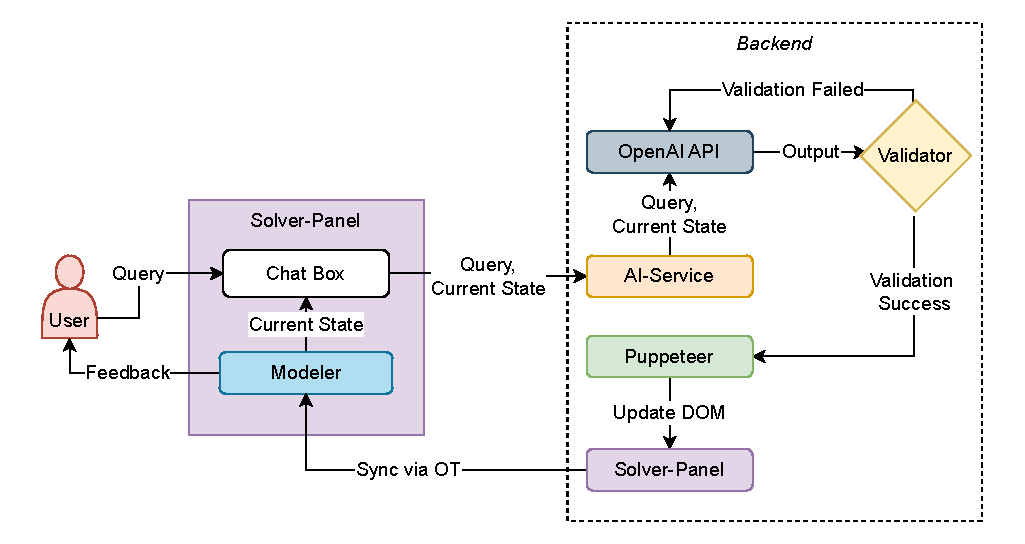
\includegraphics[width=10cm]{static/new.pdf}
  \caption{Overview of the proposed LLM architecture.}
  \label{fig:architecture}
\end{figure}


\chapter{Implementation}
In this chapter, we move from the conceptual design to the concrete implementation of the proposed architecture. We discuss the technologies and frameworks employed, how the individual components are interconnected, and the design decisions made during implementation. 

\section{High-Level System Architecture}
\subsection{Overview}
The primary access point of the Optimization Modeler platform is the \textbf{Solver-Panel}, which is implemented as an Angular application. It is responsible for core functionalities such as user authentication, model creation and editing, and multi-user collaboration. The Solver-Panel communicates with the backend service introduced in this work, which hosts the AI agent and the auxiliary services required to support the proposed architecture.

User interaction with the AI agent takes place through a chat interface embedded within the Angular application. When the user submits a prompt via this chat interface, the request is sent to the backend API service using HTTP-based communication.

\subsection{Class Hierarchy}
We now describe the concrete classes involved in the architecture. The \textbf{Solver-Panel} class provides the frontend interface of the Optimization Modeler. On the backend, we implement an Express.js-based service referred to as the \textbf{AI-Agent} service. This service consists of two main components. The first is the \textbf{LLM} service, which provides an abstraction layer for interacting with large language models—in our case, OpenAI’s GPT-based models—through their API. The second component is the \textbf{Puppeteer-Controller}, which is responsible for controlling a server-side browser instance using the Puppeteer automation framework. This controller enables the AI agent to interact with the Optimization Modeler by programmatically accessing and manipulating the Document Object Model (DOM).


\section{Solver-Panel Frontend}
This section describes the user-facing component of the Optimization Platform, referred to as the \emph{Solver-Panel}, and its integration with the AI agent service.

\subsection{User Authentication}
Users begin by creating an account and authenticating via the Solver-Panel's dedicated security layer. This infrastructure manages user sessions and access control for various optimization workspaces. The underlying authentication workflows and the management of user identities are implemented following the architecture established by Begaj \cite{DeniThesisMsc}.

\subsection{Internal Modeler}
The core of the interface is the Optimization Modeler, a vanilla JavaScript module integrated into the Angular-based Solver-Panel application. Once authenticated, users can construct Mixed-Integer Linear Programs (MILPs) using an intuitive drag-and-drop interface. This visual representation is backed by a domain-specific, XML-like markup language. Any operation performed within the graphical Document Object Model (DOM) is automatically translated into this syntax, which serves as the source of truth for the optimization model \cite{MarkoThesisBsc, MaksimThesisMsc}.

\subsection{Collaboration and Agent Invitation}
The platform supports multi-user collaboration through a link-sharing architecture. Users can generate and share session links that allow others to join a workspace with either read-only or editing privileges \cite{MarkoThesisMsc}. To facilitate AI assistance, we extended this mechanism to include an ``Invite AI Agent'' functionality. 

When triggered, the frontend sends an HTTP POST request to the AI agent service's \texttt{invokeai} (or \texttt{/puppet}) endpoint. This request includes the \texttt{writeUrl} (edit link) of the current session. The backend server uses this link to launch a headless browser instance that connects to the workspace, effectively joining the session as a virtual collaborator.

\subsection{Chat Interface and Request Processing}

To enable natural language interaction, the modeler includes a dedicated chat interface. When a user submits a query, the frontend invokes the agent's \texttt{processrequest} (or \texttt{/openai}) API endpoint. The payload for this request consists of two primary components: the current state of the optimization model (extracted in its XML format) and the user's natural language prompt. The agent service then leverages a Large Language Model to interpret the request within the context of the existing model, generating the necessary modifications which are subsequently applied back to the workspace.


\section{Browser Automation Layer}
\subsection{Initialization}
When the API endpoint \texttt{invokeAI} is called, the \texttt{puppetInit()} method of the Puppeteer controller is executed first. This method launches an instance of a headless browser (Google Chrome) on the server, navigates to the login page of the Optimization Modeler, enters the authentication credentials associated with the AI user, and completes the login process.

After the AI user has successfully authenticated, Puppeteer is used again to navigate to the \texttt{editURL} received in the response body. Visiting this URL opens the shared instance of the optimization model within the browser. Since this browser instance runs on the backend server, the shared modeler instance can now be accessed and manipulated programmatically through the backend.


\subsection{DOM Manipulation}
This layer is responsible for handling DOM manipulation by leveraging the capabilities provided by the Puppeteer service. After the user submits a request through the chat interface and the LLM service generates the corresponding output, the backend accesses the \texttt{innerHTML} of the modeler instance’s document body and replaces the current model with the model generated by the LLM.

This operation triggers the same internal update mechanisms as those invoked when a human user manually modifies the model through the interface. As a result, the change is propagated automatically to all users connected to the same collaborative session, ensuring consistency across all active instances.





\section{LLM Integration}

\subsection{Context}
When a user submits a request through the chat interface, the \texttt{/openaiResponse} endpoint is invoked. This endpoint receives the current state of the optimization model along with the user’s prompt in the request body. The backend then forwards this information to the LLM as contextual input.

Providing the current state of the model allows the LLM to understand what the user is currently working on and the progress made so far. The quality and usefulness of the LLM’s output are strongly influenced by the clarity and specificity of the user prompt; consequently, more detailed prompts generally result in more accurate and helpful responses.

\subsection{Prompt Engineering}
Prompt engineering plays a crucial role in generating functional and reliable outputs from large language models. While users are encouraged to formulate prompts that clearly and precisely describe their requirements, system-level prompts must also be carefully designed.

The LLM must be explicitly instructed about its role and responsibilities. In our case, the model operates as part of an AI agent whose purpose is to assist users in creating and modifying optimization models. The system prompt therefore includes a clear description of this role, as well as the current model state and the user’s request.

In addition, the prompt may include one or more illustrative examples that demonstrate the expected input–output behavior. This approach leverages the few-shot learning capabilities of LLMs, enabling the model to better align its responses with the desired format and semantics.



%\section{Validation Engine}
%\subsection{Schema}
%\subsection{Validation Loop}

%\section{Stateful AI-Agent}




\chapter{Evaluation}

\section{Evaluation Goals}
This chapter evaluates whether the implemented AI collaborator addresses the core objectives formulated in the introduction. Specifically, the evaluation seeks to answer the following research questions:
\begin{itemize}
    \item \textbf{RQ1 (AI Generation \& Efficiency):} To what extent does the integration of an AI-based collaborator reduce the time and manual effort required to construct MILP models compared to purely manual development?
    \item \textbf{RQ2 (Validation \& Accuracy):} How accurately can the AI agent generate mathematically and syntactically valid model structures, and how effectively does the system's validation layer prevent erroneous modifications?
    \item \textbf{RQ3 (Human-in-the-Loop \& Feedback):} How effectively does the iterative human-in-the-loop feedback mechanism enable the operator to recover from AI-generated errors and converge on a correct formulation?
\end{itemize}

To answer these questions, we evaluate the system architecture using a benchmark dataset of optimization problems tested across multiple Large Language Models (LLMs) of varying sizes.

\section{Experimental Setup}
\subsection{System Configuration}
All experiments are conducted on the integrated prototype described in this thesis, using the identical execution pipeline for all tasks. To understand how the system's performance scales with the underlying intelligence of the agent, the evaluation is performed across three different LLMs accessed via OpenRouter, representing small, medium, and large model classes. Each run uses the same system-prompt contract and identical tool availability to ensure configuration consistency.

The runtime environment consists of the modeler web client session, a LangGraph-backed orchestration runtime for threaded inference \cite{langchainLangGraph}, and a browser-automation service using Puppeteer for model read/write operations \cite{pptrPuppeteerPuppeteer}.

\subsection{Dataset and Task Design}
Instead of relying on a user study, the evaluation employs a dataset-driven benchmarking approach. The dataset consists of 10 representative MILP modeling tasks:
\begin{itemize}
    \item \textbf{7 Easy Problems:} Standard formulations (e.g., simple Knapsack, Diet Problem) requiring fewer variables and constraints.
    \item \textbf{3 Hard Problems:} Complex formulations (e.g., Facility Location, Multi-commodity Flow) requiring advanced structural adjustments and multiple interacting constraints.
\end{itemize}

For each problem in the dataset, two execution modes are measured:
\begin{enumerate}
    \item \textbf{Manual mode:} The operator models the problem entirely through direct UI interaction.
    \item \textbf{AI-assisted mode:} The operator models the problem with the AI collaborator through natural-language requests, providing iterative feedback when necessary.
\end{enumerate}

\subsection{Evaluation Procedure}
For each sample problem, the operator attempts to generate a correct, feasible model using both modes. During the AI-assisted mode, the initial prompt is provided, and the system's first generated output is evaluated. If the model is incorrect or syntactically invalid, the operator provides corrective natural-language feedback until a valid model is achieved. 

Throughout this process, the following data points are recorded: manual modeling time, AI modeling time, first-go correctness, validation layer interventions, and the number of feedback iterations required.

\section{Evaluation Metrics}

\subsection{Efficiency Metrics (RQ1)}
\begin{itemize}
    \item \textbf{Manual Modeling Time:} Total time required to manually build the model.
    \item \textbf{AI-Assisted Modeling Time:} Total time required to build the model using the AI, including prompt writing and review time.
    \item \textbf{Speedup Factor:} The ratio of manual time to AI-assisted time.
\end{itemize}

\subsection{Accuracy and Validation Metrics (RQ2)}
\begin{itemize}
    \item \textbf{First-Go Correctness:} The percentage of tasks where the AI generated a mathematically correct and syntactically valid model on its first attempt.
    \item \textbf{Validation Catch Rate:} The number of times the system's validation layer successfully intercepted and blocked an invalid or hallucinated artifact before it could corrupt the workspace.
\end{itemize}

\subsection{Human-in-the-Loop Metrics (RQ3)}
\begin{itemize}
    \item \textbf{Correction Iterations:} For models not correct on the first go, the average number of additional human-feedback prompts required to fix the errors.
    \item \textbf{Final Success Rate:} The percentage of tasks successfully completed after iterative human refinement.
\end{itemize}

\section{Results}
\subsection{RQ1: AI Generation \& Efficiency}
To answer RQ1, we compare the manual and AI-assisted completion times across the easy and hard datasets for the different LLMs.

\begin{table}[h]
\centering
\caption{Efficiency comparison across model sizes and task complexities.}
\label{tab:rq1_efficiency}
\begin{tabular}{lcccc}
\hline
\textbf{Model Size} & \textbf{Task Level} & \textbf{Manual Time (avg)} & \textbf{AI Time (avg)} & \textbf{Speedup} \\
\hline
Small LLM & Easy (7) & -- & -- & -- \\
Small LLM & Hard (3) & -- & -- & -- \\
Medium LLM & Easy (7) & -- & -- & -- \\
Medium LLM & Hard (3) & -- & -- & -- \\
Large LLM & Easy (7) & -- & -- & -- \\
Large LLM & Hard (3) & -- & -- & -- \\
\hline
\end{tabular}
\end{table}

Table~\ref{tab:rq1_efficiency} presents the core efficiency metrics recorded during the evaluation. The \textit{Manual Time} serves as the baseline, representing the operator's speed when using the platform without AI assistance. The \textit{AI Time} captures the end-to-end duration from submitting the initial natural language prompt to the final acceptance of the model, including any necessary review or wait times. The \textit{Speedup} factor is calculated as the ratio of manual time to AI time. A speedup factor greater than 1.0 indicates that the AI collaborator successfully accelerated the modeling process. By categorizing the results into Easy and Hard tasks, this table allows us to observe whether the efficiency gains are consistent across varying levels of problem complexity, and whether larger, slower LLMs negatively impact overall modeling speed due to high inference latency.

\subsection{RQ2: Validation \& Accuracy}
To answer RQ2, we measure the system's ability to generate valid models on the first attempt and the effectiveness of the validation layer in intercepting errors.

\begin{table}[h]
\centering
\caption{First-go accuracy and validation performance across LLMs.}
\label{tab:rq2_accuracy}
\begin{tabular}{lccc}
\hline
\textbf{Model Size} & \textbf{First-Go Correct (\%)} & \textbf{Caught by Val.} & \textbf{Uncaught Errors} \\
\hline
Small LLM & -- & -- & -- \\
Medium LLM & -- & -- & -- \\
Large LLM & -- & -- & -- \\
\hline
\end{tabular}
\end{table}

The metrics in Table~\ref{tab:rq2_accuracy} illustrate the raw generation capability and safety of the architecture. \textit{First-Go Correct (\%)} indicates the proportion of tasks where the AI successfully generated a fully valid and mathematically accurate model without requiring any human intervention. When the model failed to produce a correct formulation on the first attempt, the errors were either intercepted by the system or reached the user. \textit{Caught by Val.} tracks the number of times the architectural validation layer successfully identified and blocked syntactically invalid or hallucinated artifacts, proving the effectiveness of the system's safety mechanisms. Conversely, \textit{Uncaught Errors} represents logical flaws that bypassed technical validation and required human identification, directly informing the necessity of the human-in-the-loop workflow evaluated in the next section.

\subsection{RQ3: Human-in-the-Loop \& Feedback}
To answer RQ3, we analyze the correction overhead required when the AI fails to produce a correct model initially.

\begin{table}[h]
\centering
\caption{Iterative correction cycles required to achieve a valid model.}
\label{tab:rq3_hitl}
\begin{tabular}{lccc}
\hline
\textbf{Model Size} & \textbf{Avg. Corrections} & \textbf{Max Iterations} & \textbf{Final Success (\%)} \\
\hline
Small LLM & -- & -- & -- \\
Medium LLM & -- & -- & -- \\
Large LLM & -- & -- & -- \\
\hline
\end{tabular}
\end{table}

Table~\ref{tab:rq3_hitl} evaluates the effectiveness of the iterative feedback mechanism for the subset of tasks that were not solved correctly on the first attempt. The \textit{Avg. Corrections} metric tracks the average number of follow-up prompts the operator had to provide to guide the AI toward a correct solution. A low average indicates that the AI agent successfully maintains context and incorporates human feedback efficiently. \textit{Max Iterations} highlights the worst-case scenario encountered during testing, indicating potential failure states or "prompt loops." Finally, the \textit{Final Success (\%)} demonstrates the ultimate reliability of the platform; it shows the percentage of tasks that were eventually solved correctly when combining the AI's generation capabilities with human supervision, regardless of initial failures.

\section{Threats to Validity}
\subsection{Internal Validity}
The evaluation relies on a predefined dataset of optimization problems. The prompts used to describe these problems may contain implicit biases based on the operator's formulation style. To mitigate this, standard problem descriptions from optimization literature are used where possible.

\subsection{External Validity}
The 10 selected problems represent a subset of possible MILP formulations and may not generalize to highly specific industrial applications. Furthermore, \textbf{LLM Bias} acts as a significant threat to external validity: the architecture's output quality is inherently bounded by the capabilities of the underlying LLMs. While testing across three model sizes mitigates this by showing performance variance, future advancements or regressions in LLM capabilities will directly impact the measured efficiency and accuracy of the platform.

\subsection{Construct Validity}
Measuring efficiency via time comparison assumes the manual operator is proficient. Differences in the operator's manual modeling speed could skew the speedup factor.

\section{Summary}
This chapter introduced a dataset-driven evaluation methodology to assess the proposed AI collaborator. By benchmarking 10 optimization tasks across three different LLM sizes, the evaluation provides quantitative insights into the system's efficiency gains (RQ1), architectural accuracy and safety (RQ2), and the effectiveness of the human-in-the-loop feedback mechanism for error recovery (RQ3).
\chapter{Conclusion}
\section{Summary}
This thesis has presented a novel architecture for integrating an AI agent as a "first-class collaborator" within a web-based Optimization Platform. By bridging the gap between natural language processing and visual modeling, the proposed system addresses the core challenges of inefficiency and high entry barriers in Mixed-Integer Linear Programming (MILP).

The primary technical contribution of this work is the "Phantom User" paradigm. By utilizing a headless browser automation layer (Puppeteer), the AI agent is able to join collaborative modeling sessions as a virtual participant. This approach leverages the platform's existing Operational Transformation (OT) infrastructure, ensuring that AI-driven modifications are synchronized in real-time across all connected clients without requiring invasive changes to the legacy backend.

To ensure the reliability of the system, we implemented a multi-layered safety framework. A dedicated validation layer enforces syntactic and structural correctness of the LLM-generated XML-like markup, effectively mitigating the risk of model corruption due to hallucinations. Furthermore, a stateful "Human-in-the-Loop" workflow ensures that the user remains the ultimate authority, providing a mechanism for iterative feedback and final approval of all agent-led changes.

In conclusion, this work demonstrates that AI agents can move beyond being simple "tools" to become active, collaborative participants in complex technical domains, significantly enhancing the accessibility and productivity of optimization modeling.

\section{Current Status and Next Steps}
While the theoretical architecture has been established, the implementation is currently in a functional prototype stage. This section outlines the current capabilities and the prioritized milestones for future development.

\subsection{Implementation Status}
The core communication pipeline between the \emph{Solver-Panel} frontend and the \emph{AI-Agent} backend service is fully operational. A dedicated chat interface has been integrated into the modeler, enabling natural language interaction. Currently, the backend service successfully utilizes Puppeteer to join collaborative sessions and the OpenAI API to translate user prompts into model updates. The agent is capable of perceiving the model state, generating modifications, and applying them directly to the Document Object Model (DOM) of the shared workspace.

\subsection{Future Milestones}
To reach the final vision of a robust and secure collaborative environment, the following components are currently under development:

\begin{itemize}
    \item \textbf{Human-in-the-Loop Implementation:} The current version applies changes directly to the model. The next phase involves implementing the full iterative feedback loop (Accept/Reject/Refine) using a stateful framework like LangGraph. This will ensure that all AI-driven modifications remain tentative until they receive explicit user approval.
    
    \item \textbf{Schema-Based Validation:} Work is ongoing to define a formal grammar for the platform's XML-like syntax. This schema will form the basis of the validation layer, allowing the agent to detect and correct "hallucinations" or syntax errors before they are presented to the user.
    
    \item \textbf{UI/UX Enhancements:} To improve the collaborative experience, further UI features will be added to provide the user with clear visual cues regarding the agent’s current state (e.g., "Thinking," "Validating," or "Awaiting Review").
\end{itemize}



\cleardoublepage
\printbibliography[heading=bibintoc]

\clearpage
\appendix
\chapter{Implementation File Structure}
\label{sec:appendix-filestructure}

This appendix provides an implementation-oriented file map for the AI collaborator architecture described in the main chapters. The listing focuses on the modules that are directly relevant for invitation flow, chat runtime, orchestration, and browser automation.

\section{High-Level Repository Layout}
\begingroup
\footnotesize
\begin{verbatim}
optimization-platform/
├── Solver-Panel/
│   └── src/app/functions/internal-modeler/
│       ├── internal-modeler.component.ts
│       └── internal-modeler.component.html
├── Modeler/
│   ├── src/
│   │   ├── modeler.js
│   │   ├── mountAIAgent.jsx
│   │   └── ModalAIAgent.tsx
│   └── lib/
│       └── chatApi.ts
├── AI-Collaborator/
│   └── server/
│       ├── src/agent.py
│       ├── main.py
│       └── pyproject.toml
└── Ai-Agent/
    ├── index.js
    ├── puppet.js
    └── openai.js
\end{verbatim}

\section{File Responsibilities}
\begin{itemize}
    \item \textbf{\texttt{internal-modeler.component.ts/.html}}: Adds and wires the ``Invite AI Agent'' interaction and collaboration link handoff from frontend to automation bridge.
    \item \textbf{\texttt{modeler.js}}: Hosts modeler runtime behavior and exposes model state access methods used by the assistant integration.
    \item \textbf{\texttt{mountAIAgent.jsx}, \texttt{ModalAIAgent.tsx}}: Mount and run the embedded assistant-ui chat modal and bind runtime callbacks.
    \item \textbf{\texttt{chatApi.ts}}: Implements thread creation, state retrieval, and streaming requests to the LangGraph runtime API.
    \item \textbf{\texttt{agent.py}}: Defines LangGraph state graph, tool nodes, prompt contract, and interrupt-based HITL flow.
    \item \textbf{\texttt{main.py}}: Exposes Python service entrypoints and API wiring.
    \item \textbf{\texttt{index.js}}: Node/Express bridge endpoints (\texttt{/puppet}, \texttt{/update-html}, \texttt{/get-html}).
    \item \textbf{\texttt{puppet.js}}: Puppeteer lifecycle and direct modeler DOM read/write execution.
    \item \textbf{\texttt{openai.js}}: LLM-side helper path used by Node bridge flows.
\end{itemize}

\section{Cross-Module Execution Path}
The operational call chain spans the listed modules as follows:
\begin{enumerate}
    \item Frontend invitation and chat interaction start in \texttt{Solver-Panel} and \texttt{Modeler}.
    \item Runtime messages are forwarded to the orchestration layer in \texttt{AI-Collaborator/server}.
    \item Tool calls are delegated to Node endpoints in \texttt{Ai-Agent/index.js}.
    \item Puppeteer methods in \texttt{puppet.js} apply updates to the active modeler DOM.
    \item Updated state propagates back to all collaborators through the platform's existing collaboration channel.
\end{enumerate}

% Further appendices can be added as separate chapters: \chapter{Second Appendix}
% Appendices (or any other elements within those) can be referenced as usual with \cref.

\chapter{API Endpoint Reference}
\label{sec:appendix-api-endpoints}

This appendix documents the API surfaces used by the implemented AI-collaboration pipeline. It includes the Node automation bridge endpoints, the LangGraph runtime operations used by the frontend, and the currently exposed FastAPI endpoints in the Python service.

\section{Node Automation Bridge (Ai-Agent)}
\label{sec:appendix-api-node-bridge}

\begin{itemize}
    \item \textbf{\texttt{POST /puppet}} \\
    Payload: \texttt{\{"link": <writeUrl>\}} \\
    Purpose: Initializes Puppeteer session and joins collaborative workspace via write URL. \\
    Response: Confirmation text.

    \item \textbf{\texttt{POST /update-html}} \\
    Payload: \texttt{\{"newHTML": <markup>\}} \\
    Purpose: Applies generated model markup to active modeler instance in browser session. \\
    Response: Success flag.

    \item \textbf{\texttt{GET /get-html}} \\
    Payload: none \\
    Purpose: Retrieves current modeler instance markup from active browser session. \\
    Response: Current HTML payload.

    \item \textbf{\texttt{POST /openai}} \\
    Payload: \texttt{\{"currentModel": ..., "userPrompt": ...\}} \\
    Purpose: Alternate Node-side generation path; generates and applies an update. \\
    Response: Success flag.

    \item \textbf{\texttt{GET /}} \\
    Payload: none \\
    Purpose: Health/check endpoint used for basic service availability checks.
\end{itemize}

\section{LangGraph Runtime API Operations (Frontend Usage)}
\label{sec:appendix-api-langgraph}

The frontend uses the \texttt{@langchain/langgraph-sdk} client against the configured runtime URL (\texttt{http://127.0.0.1:2024}) through thread/run operations:

\begin{itemize}
    \item \textbf{\texttt{threads.create()}} \\
    Input: none \\
    Purpose: Creates a new persistent thread and returns thread identifier used by assistant runtime.

    \item \textbf{\texttt{threads.getState(threadId)}} \\
    Input: \texttt{threadId} \\
    Purpose: Loads persisted message state and pending interrupt metadata for chat resume.

    \item \textbf{\texttt{runs.stream(threadId, assistantId, ...)}} \\
    Input: \texttt{input.messages}, optional \texttt{command}, \texttt{streamMode} \\
    Purpose: Starts a streamed run for a thread and returns incremental model outputs and state updates (messages/updates stream).
\end{itemize}

\section{Python FastAPI Service Endpoints}
\label{sec:appendix-api-python}

The Python service currently exposes minimal endpoints in \texttt{AI-Collaborator/server/main.py}:

\begin{itemize}
    \item \textbf{\texttt{GET /}} \\
    Purpose: Basic root endpoint returning static payload (service scaffold/health check).

    \item \textbf{\texttt{POST /agent-response}} \\
    Payload: \texttt{AgentRequest\{query: str\}} \\
    Purpose: Receives agent request and currently returns static payload (placeholder endpoint).
\end{itemize}

\chapter{System Prompt Specification}
\label{sec:appendix-system-prompt}

This appendix records the system-prompt specification used by the AI orchestration service for optimization-model generation.Beyond role definition, this prompt encodes several reliability mechanisms. It includes strict structural and validation constraints (mandatory blocks, allowed child tags, and forbidden nesting patterns) so that generated outputs remain compatible with the modeler's expected schema. 

It also prescribes a deterministic execution order for generation (identify entities, define data, then construct model blocks), which reduces ambiguity in complex prompts. In addition, the prompt design supports example-based in-context guidance (one-shot and few-shot style examples), enabling the model to align with desired input-output behavior without retraining.

\begin{verbatim}
## Role and Objective
You are an expert Mathematical Programming Assistant. Your specific task is to
translate natural language problem descriptions into the "Markup Language for MIPs".

You must act as both a mathematical translator and a syntax specialist. You
will output valid XML-style markup adhering strictly to the grammar and
validation rules defined below.

## Core Language Rules
1. Hyphen Suffix: Every single tag MUST end with a hyphen
   (e.g., <model->, <con->, <var->, <each->).
2. Root Structure: Every output must be wrapped in an <instance-> tag.
   An instance can contain AT MOST ONE <model-> tag, but may contain
   MULTIPLE <data-> tags.
3. Mandatory Model Blocks: The <model-> tag MUST contain EXACTLY ONE of
   each: <variables->, <constraints->, and <objectives->.
4. Implicit Summation: Child elements of <obj-> and <con-> are interpreted
   as a sum by default.
5. JavaScript Data: The <data-> section must contain a <script-> tag where
   sets and parameters are defined using standard JavaScript.

## Strict Grammar, Validations, and Allowed Attributes
### 1. Structural Tags
- <model->:
  - Must contain exactly one <objectives->, <constraints->, <variables->.
  - Attribute: src
- <data->:
  - Must contain <each-> or <script->.
  - Attribute: src
- <variables->:
  - Allowed children: <var->, <each->, <script->
  - Validation critical: cannot contain <con-> or <obj->
- <constraints->:
  - Allowed children: <con->, <each->, <script->
  - Validation critical: cannot contain <obj->
- <objectives->:
  - Allowed children: <obj->, <each->, <script->
  - Validation critical: cannot contain <con->

### 2. Core MIP Elements
- <obj->:
  - Allowed children: <var->, <add->, <mul->, <constant->, <each->, <script->
  - Validation critical: cannot contain another <obj->
  - Attributes in objectives:
    name, sense, weight, priority, absTol, relTol, index
  - Attributes if inside a variable: name, coefficient
- <con->:
  - Allowed children: <var->, <add->, <mul->, <constant->, <each->, <script->
  - Validation critical: cannot contain another <con->
  - Attributes in constraints: name, lb, ub, index
  - Do NOT use <lhs> or <rhs> tags
  - Attributes if inside a variable: name, coefficient
- <var->:
  - Allowed children (only if in variables): <obj->, <con->
  - Attributes in variables: name, integer, lb, ub, index
  - Attributes if inside constraint/objective: name, index, coefficient

### 3. Mathematical Statements
- <add-> and <mul->:
  - Allowed children:
    <var->, <constant->, <add->, <mul->, <each->, <script->
  - Attribute: coefficient
- <constant->:
  - No children
  - Attributes: name, value, index, coefficient

### 4. Feature Tags
- <each->:
  - Attributes: family, item, index, coefficient, if
- <script->:
  - Validation critical: cannot have 'modified' without 'src' or 'data-definition'
  - Attributes: src, data-definition, modified

## Execution Instructions
1. Identify sets, parameters, decision variables, objective function,
   constraints.
2. Draft the <data-> section with JavaScript arrays/variables in a
   <script-> tag.
3. Construct the <model-> section ensuring variables are defined before use.
4. Check output against validation-critical rules.
5. Return ONLY valid <instance-> markup (no markdown fences).

## Example Output Format
<instance->
  <model->
    <objectives->
      <obj- name="TotalCost" sense="minimize">
        <each- item="i" family="Items">
          <var- name="x" index="i" coefficient="cost[i]"></var->
        </each->
      </obj->
    </objectives->
    <constraints->
      <each- item="j" family="Bins">
        <con- name="Capacity" index="j" ub="capacity[j]">
          <each- item="i" family="Items">
            <var- name="x" index="[i,j]"></var->
          </each->
        </con->
      </each->
    </constraints->
    <variables->
      <each- item="i" family="Items">
        <each- item="j" family="Bins">
          <var- name="x" index="[i,j]" lb="0" ub="1" integer></var->
        </each->
      </each->
    </variables->
  </model->
  <data->
    <script->
      let Items = [1, 2, 3];
      let Bins = ['A', 'B'];
      let cost = [10, 20, 30];
      let capacity = {'A': 50, 'B': 50};
    </script->
  </data->
</instance->
\end{verbatim}
\endgroup

% further appendix items (such as a glossary etc., if you have them) go here

\end{document}